\section{RFC-0008: Session Data
Protocol}\label{rfc-0008-session-data-protocol}

\begin{itemize}
\tightlist
\item
  \textbf{RFC Number:} 0008
\item
  \textbf{Title:} Session Data Protocol
\item
  \textbf{Status:} Implementation
\item
  \textbf{Author(s):} Tino Breddin (@tolbrino), Lukas Pohanka
  (@NumberFour8)
\item
  \textbf{Created:} 2025-08-15
\item
  \textbf{Updated:} 2025-09-05
\item
  \textbf{Version:} v0.1.0 (Draft)
\item
  \textbf{Supersedes:} N/A
\item
  \textbf{Related Links:}
  \href{../RFC-0002-mixnet-keywords/0002-mixnet-keywords.md}{RFC-0002},
  \href{../RFC-0004-hopr-packet-protocol/0004-hopr-packet-protocol.md}{RFC-0004},
  \href{../RFC-0009-session-start-protocol/0009-session-start-protocol.md}{RFC-0009}
\end{itemize}

\subsection{1. Abstract}\label{1-abstract}

This RFC specifies the HOPR Session Data Protocol, which provides
reliable and unreliable data transmission capabilities over the HOPR
mixnet. The protocol implements TCP-like {[}01{]} features including
message segmentation, reassembly, acknowledgement, and retransmission
while maintaining simplicity and efficiency. This protocol works in
conjunction with the HOPR Session Start Protocol (see
\href{../RFC-0009-session-start-protocol/0009-session-start-protocol.md}{RFC-0009})
to provide complete session management capabilities for applications
within the HOPR mixnet ecosystem.

\subsection{2. Motivation}\label{2-motivation}

The HOPR mixnet uses HOPR packets
\href{../RFC-0004-hopr-packet-protocol/0004-hopr-packet-protocol.md}{RFC-0004}
to send data between nodes. This fundamental packet sending mechanisms
however works, similar to UDP {[}03{]}, as a fire-and-forget mechanisms
and does not provide any higher-level features any application developer
would expect. To ease adoption a HOPR node needs a way for existing
applications to use it without having to implement TCP {[}01{]} or UDP
all over again. Since HOPR protocol is not IP-based, such implementation
would require IP protocol emulation.

The HOPR Session Data Protocol fills that gap by providing reliable and
unreliable data transmission capabilities to applications. Session
establishment and lifecycle management is handled by the HOPR Session
Start Protocol
\href{../RFC-0009-session-start-protocol/0009-session-start-protocol.md}{RFC-0009},
while this protocol focuses exclusively on data transmission.

\subsection{3. Terminology}\label{3-terminology}

\begin{itemize}
\item
  \textbf{Frame}: A logical unit of data transmission in the Session
  Protocol. Frames can be of arbitrary length and are identified by a
  unique Frame ID.
\item
  \textbf{Segment}: A fixed-size fragment of a frame. Frames are split
  into segments for transmission, with each segment carrying metadata
  about its position within the frame.
\item
  \textbf{Frame ID}: A 32-bit unsigned integer that uniquely identifies
  a frame within a session (1-indexed). Frame ID values are interpreted
  as big-endian unsigned integers.
\item
  \textbf{Sequence Number (SeqNum)}: An 8-bit unsigned integer
  indicating a segment\textquotesingle s position within its frame
  (0-indexed).
\item
  \textbf{Sequence Flags (SeqFlags)}: An 8-bit value encoding additional
  segment sequence metadata.
\item
  \textbf{Session Socket}: The endpoint abstraction that implements the
  Session Protocol, available in both reliable and unreliable variants.
\item
  \textbf{MTU (Maximum Transmission Unit)}: The maximum size of a single
  HOPR protocol message, denoted as \texttt{C} throughout this
  specification.
\item
  \textbf{Terminating Segment}: A special segment that signals the end
  of a session.
\end{itemize}

\subsection{4. Specification}\label{4-specification}

\subsubsection{4.1 Protocol Overview}\label{41-protocol-overview}

The HOPR Session Data Protocol operates at version 1 and consists of
three message types that work together to provide reliable or unreliable
data transmission:

\begin{enumerate}
\def\labelenumi{\arabic{enumi}.}
\tightlist
\item
  \textbf{Segment Messages}: Carry actual data fragments
\item
  \textbf{Retransmission Request Messages}: Request missing segments
\item
  \textbf{Frame Acknowledgement Messages}: Confirm successful frame
  receipt
\end{enumerate}

The protocol supports two operational modes:

\begin{itemize}
\tightlist
\item
  \textbf{Unreliable Mode}: Fast, stateless operation similar to UDP
  {[}03{]}
\item
  \textbf{Reliable Mode}: Stateful operation with acknowledgements and
  retransmissions
\end{itemize}

Session establishment and lifecycle management is handled by the HOPR
Session Start Protocol. All multi-byte integer fields use network byte
order (big-endian) encoding to ensure consistent interpretation across
different architectures.

\subsubsection{4.2 Session Data Protocol Message
Format}\label{42-session-data-protocol-message-format}

All Session Data Protocol messages follow a common structure:

\pandocbounded{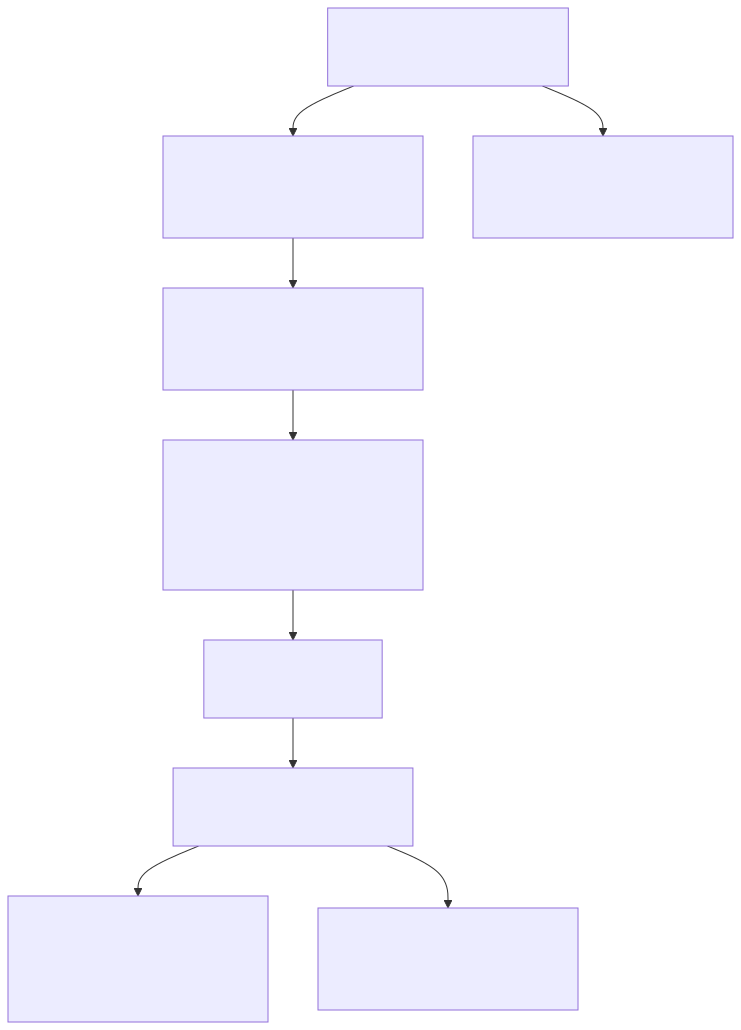
\includegraphics[keepaspectratio,width=\maxwidth,alt={Mermaid Diagram 1}]{generated/0008-session-protocol/mermaid_1.png}}

\begin{longtable}[]{@{}llll@{}}
\toprule\noalign{}
Field & Size & Description & Value \\
\midrule\noalign{}
\endhead
\bottomrule\noalign{}
\endlastfoot
\textbf{Version} & 1 byte & Protocol version & MUST be \texttt{0x01} for
version 1 \\
\textbf{Type} & 1 byte & Message type discriminant & See Message Types
table below \\
\textbf{Length} & 2 bytes & Payload length in bytes & Maximum is
\texttt{C\ -\ 4} \\
\textbf{Payload} & Variable & Message-specific data & Format depends on
message type \\
\end{longtable}

\paragraph{4.2.1 Message Types}\label{421-message-types}

\begin{longtable}[]{@{}lll@{}}
\toprule\noalign{}
Type Code & Name & Description \\
\midrule\noalign{}
\endhead
\bottomrule\noalign{}
\endlastfoot
\texttt{0x00} & Segment & Carries actual data fragments \\
\texttt{0x01} & Retransmission Request & Requests missing segments \\
\texttt{0x02} & Frame Acknowledgement & Confirms successful frame
receipt \\
\end{longtable}

\paragraph{4.2.2 Byte Order}\label{422-byte-order}

All multi-byte integer fields and values in the Session Data Protocol
MUST be encoded and interpreted in network byte order (big-endian). This
applies to:

\textbf{Protocol Message Fields:}

\begin{itemize}
\tightlist
\item
  \textbf{Length} field (2 bytes) in the common message format
\item
  \textbf{Frame ID} field (4 bytes) in Segment, Retransmission Request,
  and Frame Acknowledgement messages
\item
  Any future numeric fields added to the protocol
\end{itemize}

This requirement ensures consistent interpretation across different
architectures and prevents interoperability issues between
implementations.

\subsubsection{4.3 Segment Message}\label{43-segment-message}

\paragraph{4.3.1 Segment Structure}\label{431-segment-structure}

\pandocbounded{\includegraphics[keepaspectratio,width=\maxwidth,alt={Mermaid Diagram 2}]{generated/0008-session-protocol/mermaid_2.png}}

\begin{longtable}[]{@{}llll@{}}
\toprule\noalign{}
Field & Size & Description & Valid Range \\
\midrule\noalign{}
\endhead
\bottomrule\noalign{}
\endlastfoot
\textbf{Frame ID} & 4 bytes & Frame identifier & 1 to 4,294,967,295 \\
\textbf{Sequence Number} & 1 byte & Segment position within frame
(0-based) & 0-63 \\
\textbf{Sequence Flags} & 1 byte & Segment metadata flags & See Sequence
Flags table below \\
\textbf{Segment Data} & Variable & Payload data & 0 to
(\texttt{C\ -\ 10}) bytes \\
\end{longtable}

\paragraph{4.3.2 Sequence Flags Bitmap}\label{432-sequence-flags-bitmap}

\begin{longtable}[]{@{}llll@{}}
\toprule\noalign{}
Bit & Flag Name & Description & Values \\
\midrule\noalign{}
\endhead
\bottomrule\noalign{}
\endlastfoot
7 & \textbf{Termination Flag} & Indicates terminating segment &
\texttt{0} = Normal, \texttt{1} = Terminating \\
6 & \textbf{Reserved} & Reserved for future use & MUST be \texttt{0} \\
5-0 & \textbf{Segment Count} & Total segments in frame minus 1 &
\texttt{0}-\texttt{63} (1-64 segments) \\
\end{longtable}

\paragraph{4.3.3 Segmentation Rules}\label{433-segmentation-rules}

\begin{longtable}[]{@{}lll@{}}
\toprule\noalign{}
Rule & Requirement & Description \\
\midrule\noalign{}
\endhead
\bottomrule\noalign{}
\endlastfoot
\textbf{Segmentation Threshold} & MUST & Frames MUST be segmented when
larger than \texttt{(C\ -\ 10)} bytes \\
\textbf{Maximum Segments} & MUST & Maximum 64 segments per frame (6-bit
sequence length field limit) \\
\textbf{Segment Sizing} & SHOULD & Each segment except the last SHOULD
be of equal size \\
\textbf{Empty Segments} & MUST & Empty segments MUST be valid (used for
terminating segments) \\
\textbf{Frame ID Ordering} & MUST & Frame IDs MUST be monotonically
increasing within a session \\
\end{longtable}

\paragraph{4.3.4 Protocol Constants}\label{434-protocol-constants}

\begin{longtable}[]{@{}lll@{}}
\toprule\noalign{}
Constant & Value & Description \\
\midrule\noalign{}
\endhead
\bottomrule\noalign{}
\endlastfoot
\textbf{Protocol Version} & \texttt{0x01} & Current protocol version \\
\textbf{Segment Overhead} & 10 bytes & Header overhead per segment (4
common + 6 segment) \\
\textbf{Maximum Frame ID} & 4,294,967,295 & Maximum 32-bit frame
identifier \\
\textbf{Maximum Segments} & 64 & Maximum segments per frame \\
\textbf{Maximum Payload Length} & \texttt{C\ -\ 4} bytes & Maximum
message payload size \\
\end{longtable}

\subsubsection{4.4 Retransmission Request
Message}\label{44-retransmission-request-message}

\paragraph{4.4.1 Request Structure}\label{441-request-structure}

\pandocbounded{\includegraphics[keepaspectratio,width=\maxwidth,alt={Mermaid Diagram 3}]{generated/0008-session-protocol/mermaid_3.png}}

The message contains a sequence of 5-byte entries:

\begin{longtable}[]{@{}llll@{}}
\toprule\noalign{}
Field & Size & Description & Format \\
\midrule\noalign{}
\endhead
\bottomrule\noalign{}
\endlastfoot
\textbf{Frame ID} & 4 bytes & Frame identifier & 1 to 4,294,967,295 \\
\textbf{Missing Bitmap} & 1 byte & Bitmap of missing segments & See
Missing Bitmap table below \\
\end{longtable}

\paragraph{4.4.2 Missing Bitmap Format}\label{442-missing-bitmap-format}

\begin{longtable}[]{@{}lll@{}}
\toprule\noalign{}
Bit & Sequence Number & Description \\
\midrule\noalign{}
\endhead
\bottomrule\noalign{}
\endlastfoot
0 & Segment 0 & \texttt{1} = Missing, \texttt{0} = Received \\
1 & Segment 1 & \texttt{1} = Missing, \texttt{0} = Received \\
2 & Segment 2 & \texttt{1} = Missing, \texttt{0} = Received \\
3 & Segment 3 & \texttt{1} = Missing, \texttt{0} = Received \\
4 & Segment 4 & \texttt{1} = Missing, \texttt{0} = Received \\
5 & Segment 5 & \texttt{1} = Missing, \texttt{0} = Received \\
6 & Segment 6 & \texttt{1} = Missing, \texttt{0} = Received \\
7 & Segment 7 & \texttt{1} = Missing, \texttt{0} = Received \\
\end{longtable}

\textbf{Note:} This message MUST be used only for frames with up to 8
segments (due to bitmap size limitation). Reliable sessions are limited
to 7 segments per frame. Unreliable sessions SHOULD not have this
limitation.

\paragraph{4.4.3 Request Rules}\label{443-request-rules}

\begin{longtable}[]{@{}lll@{}}
\toprule\noalign{}
Rule & Requirement & Description \\
\midrule\noalign{}
\endhead
\bottomrule\noalign{}
\endlastfoot
\textbf{Ordering} & MUST & Entries MUST be ordered by Frame ID
(ascending) \\
\textbf{Padding} & MAY & Frame ID of \texttt{0} indicates padding
(ignored) \\
\textbf{Entry Limit} & MUST & Maximum entries per message:
\texttt{(C\ -\ 4)\ /\ 5} \\
\textbf{Segment Limit} & MUST & Only the first 8 segments per frame can
be requested \\
\end{longtable}

\subsubsection{4.5 Frame Acknowledgement
Message}\label{45-frame-acknowledgement-message}

\paragraph{4.5.1 Acknowledgement
Structure}\label{451-acknowledgement-structure}

\pandocbounded{\includegraphics[keepaspectratio,width=\maxwidth,alt={Mermaid Diagram 4}]{generated/0008-session-protocol/mermaid_4.png}}

\begin{longtable}[]{@{}llll@{}}
\toprule\noalign{}
Field & Size & Description & Rules \\
\midrule\noalign{}
\endhead
\bottomrule\noalign{}
\endlastfoot
\textbf{Frame ID List} & 4 bytes each & List of fully received frame
identifiers & See Acknowledgement Rules table below \\
\end{longtable}

\paragraph{4.5.2 Acknowledgement Rules}\label{452-acknowledgement-rules}

\begin{longtable}[]{@{}lll@{}}
\toprule\noalign{}
Rule & Requirement & Description \\
\midrule\noalign{}
\endhead
\bottomrule\noalign{}
\endlastfoot
\textbf{Ordering} & MUST & Frame IDs MUST be in ascending order \\
\textbf{Padding} & MAY & Frame ID of \texttt{0} indicates padding
(ignored) \\
\textbf{Entry Limit} & MUST & Maximum frame IDs per message:
\texttt{(C\ -\ 4)\ /\ 4} \\
\textbf{Completeness} & MUST & Only acknowledge frames that are fully
received \\
\end{longtable}

\subsubsection{4.6 Protocol State
Machines}\label{46-protocol-state-machines}

\paragraph{4.6.1 Unreliable Socket State
Machine}\label{461-unreliable-socket-state-machine}

\pandocbounded{\includegraphics[keepaspectratio,width=\maxwidth,alt={Mermaid Diagram 5}]{generated/0008-session-protocol/mermaid_5.png}}

\paragraph{4.6.2 Reliable Socket State
Machine}\label{462-reliable-socket-state-machine}

\pandocbounded{\includegraphics[keepaspectratio,width=\maxwidth,alt={Mermaid Diagram 6}]{generated/0008-session-protocol/mermaid_6.png}}

\subsubsection{4.7 Timing and Reliability
Parameters}\label{47-timing-and-reliability-parameters}

\paragraph{4.7.1 Unreliable Mode}\label{471-unreliable-mode}

\begin{itemize}
\tightlist
\item
  No acknowledgements or retransmissions
\item
  Frames may be delivered out-of-order
\item
  No delivery guarantees
\item
  Suitable for real-time or loss-tolerant applications
\end{itemize}

\paragraph{4.7.2 Reliable Mode
Parameters}\label{472-reliable-mode-parameters}

\begin{longtable}[]{@{}llll@{}}
\toprule\noalign{}
Parameter & Default Value & Description & Requirement \\
\midrule\noalign{}
\endhead
\bottomrule\noalign{}
\endlastfoot
\textbf{Frame Timeout} & 800ms & Time before requesting retransmission &
SHOULD be configurable \\
\textbf{Acknowledgement Window} & 255 frames & Maximum unacknowledged
frames & MUST NOT exceed 255 \\
\textbf{Retransmission Limit} & 3 attempts & Maximum retransmission
attempts & Implementation-defined \\
\textbf{Acknowledgement Batching} & 100ms & Maximum delay for batching
ACKs & SHOULD be configurable \\
\end{longtable}

\subsubsection{4.8 Session Termination}\label{48-session-termination}

\begin{enumerate}
\def\labelenumi{\arabic{enumi}.}
\tightlist
\item
  Either party MAY send a terminating segment (empty segment with
  termination flag set)
\item
  Upon receiving a terminating segment:

  \begin{itemize}
  \tightlist
  \item
    Unreliable sockets SHOULD close immediately
  \item
    Reliable sockets MUST complete pending acknowledgements before
    closing
  \end{itemize}
\item
  No data frames MUST be sent after a terminating segment
\end{enumerate}

\subsubsection{4.9 Example Message
Exchanges}\label{49-example-message-exchanges}

All numeric values in the examples below are shown in their logical
representation. Frame IDs and other multi-byte integers are encoded in
big-endian format on the wire.

\paragraph{4.9.1 Simple Frame Transmission (Unreliable
Mode)}\label{491-simple-frame-transmission-unreliable-mode}

Sending a 300-byte frame with MTU=256 (246 bytes available per segment
after 10-byte overhead):

\pandocbounded{\includegraphics[keepaspectratio,width=\maxwidth,alt={Mermaid Diagram 7}]{generated/0008-session-protocol/mermaid_7.png}}

\paragraph{4.9.2 Frame with Retransmission (Reliable
Mode)}\label{492-frame-with-retransmission-reliable-mode}

Reliable transmission where the middle segment is lost and
retransmitted:

\pandocbounded{\includegraphics[keepaspectratio,width=\maxwidth,alt={Mermaid Diagram 8}]{generated/0008-session-protocol/mermaid_8.png}}

\paragraph{4.9.3 Multiple Frame Acknowledgement (Reliable
Mode)}\label{493-multiple-frame-acknowledgement-reliable-mode}

Efficiently acknowledging multiple received frames in a batch:

\pandocbounded{\includegraphics[keepaspectratio,width=\maxwidth,alt={Mermaid Diagram 9}]{generated/0008-session-protocol/mermaid_9.png}}

\paragraph{4.9.4 Session Termination (Reliable
Mode)}\label{494-session-termination-reliable-mode}

Graceful session termination with acknowledgement:

\pandocbounded{\includegraphics[keepaspectratio,width=\maxwidth,alt={Mermaid Diagram 10}]{generated/0008-session-protocol/mermaid_10.png}}

\paragraph{4.9.5 Session Termination (Unreliable
Mode)}\label{495-session-termination-unreliable-mode}

Immediate session termination without acknowledgement:

\pandocbounded{\includegraphics[keepaspectratio,width=\maxwidth,alt={Mermaid Diagram 11}]{generated/0008-session-protocol/mermaid_11.png}}

\subsection{5. Design Considerations}\label{5-design-considerations}

\subsubsection{5.1 Maximum Segments
Limitation}\label{51-maximum-segments-limitation}

The protocol limits frames to 64 segments due to the 6-bit sequence
length field. This provides a good balance between:

\begin{itemize}
\tightlist
\item
  Frame size flexibility (up to 64 × MTU)
\item
  Protocol overhead (1 byte for sequence information)
\item
  Implementation complexity (simple bitmap for retransmissions)
\end{itemize}

\subsubsection{5.2 Frame ID Space}\label{52-frame-id-space}

The 32-bit Frame ID space allows for over 4 billion frames per session.
Frame IDs MUST be monotonically increasing to enable:

\begin{itemize}
\tightlist
\item
  Duplicate detection
\item
  Out-of-order delivery handling
\item
  Simple state management
\end{itemize}

The Session MUST terminate when Frame ID of 0 is encountered by the
receiving side, indicating an overflow.

\subsubsection{5.3 Retransmission Request
Design}\label{53-retransmission-request-design}

Limiting retransmission requests to the first 8 segments per frame:

\begin{itemize}
\tightlist
\item
  Keeps message format simple (1-byte bitmap)
\item
  Covers the common case (most frames have ≤8 segments)
\item
  Frames requiring \textgreater8 segments can use smaller frame sizes
\end{itemize}

\subsubsection{5.4 Protocol Overhead}\label{54-protocol-overhead}

\begin{itemize}
\tightlist
\item
  Minimum overhead per segment: 10 bytes (4 header + 6 segment header)
\item
  Maximum protocol efficiency: (C - 10) / C
\item
  For C = 1024: \textasciitilde99\% efficiency
\item
  For C = 256: \textasciitilde96\% efficiency
\end{itemize}

\subsection{6. Compatibility}\label{6-compatibility}

\subsubsection{6.1 Version
Compatibility}\label{61-version-compatibility}

\begin{itemize}
\tightlist
\item
  Version 1 is the initial Session Data protocol version
\item
  Future versions MUST use different version numbers
\item
  Implementations MUST reject messages with unknown versions
\item
  Version negotiation is out of scope for this specification
\end{itemize}

\subsubsection{6.2 Transport
Requirements}\label{62-transport-requirements}

\begin{itemize}
\tightlist
\item
  Requires bidirectional communication channel
\item
  No assumptions about ordering or reliability
\end{itemize}

\subsection{7. Security Considerations}\label{7-security-considerations}

\subsubsection{7.1 Protocol Security}\label{71-protocol-security}

\begin{itemize}
\tightlist
\item
  The protocol provides NO encryption or authentication
\item
  Security MUST be provided by the underlying transport
\item
  Frame IDs are predictable and MUST NOT be used for security
\end{itemize}

\subsection{8. Future Work}\label{8-future-work}

\begin{itemize}
\tightlist
\item
  Enhanced acknowledgement schemes for better efficiency
\item
  Forward error correction for high-loss environments
\end{itemize}

\subsection{9. Implementation Notes}\label{9-implementation-notes}

\subsubsection{9.1 Testing
Recommendations}\label{91-testing-recommendations}

\begin{itemize}
\tightlist
\item
  Test with various MTU sizes (256, 512, 1024, 1500, 9000)
\item
  Simulate packet loss, reordering, and duplication
\item
  Verify termination handling under all conditions
\item
  Stress test with maximum frame sizes and counts
\end{itemize}

\subsection{10. References}\label{10-references}

{[}01{]} Postel, J. (1981).
\href{https://datatracker.ietf.org/doc/html/rfc793}{Transmission Control
Protocol}. \emph{IETF RFC 793}.

{[}02{]} Bormann, C. \& Hoffman, P. (2013).
\href{https://datatracker.ietf.org/doc/html/rfc7049}{Concise Binary
Object Representation (CBOR)}. \emph{IETF RFC 7049}.

{[}03{]} Postel, J. (1980).
\href{https://datatracker.ietf.org/doc/html/rfc768}{User Datagram
Protocol}. \emph{IETF RFC 768}.
